Podemos identificar que ambos algoritmos utilizan un mismo número de pasos.
Como la localidad espacial no entra en juego para ninguno de estos podemos
acelerar la ejecución fusionando ambos bucles en uno. Modificamos el código,
ejecutamos las pruebas sobre \texttt{atcgrid} y obtenemos los resultados que
mostramos en la figura A.1.

\begin{figure}[H]
    \centering
    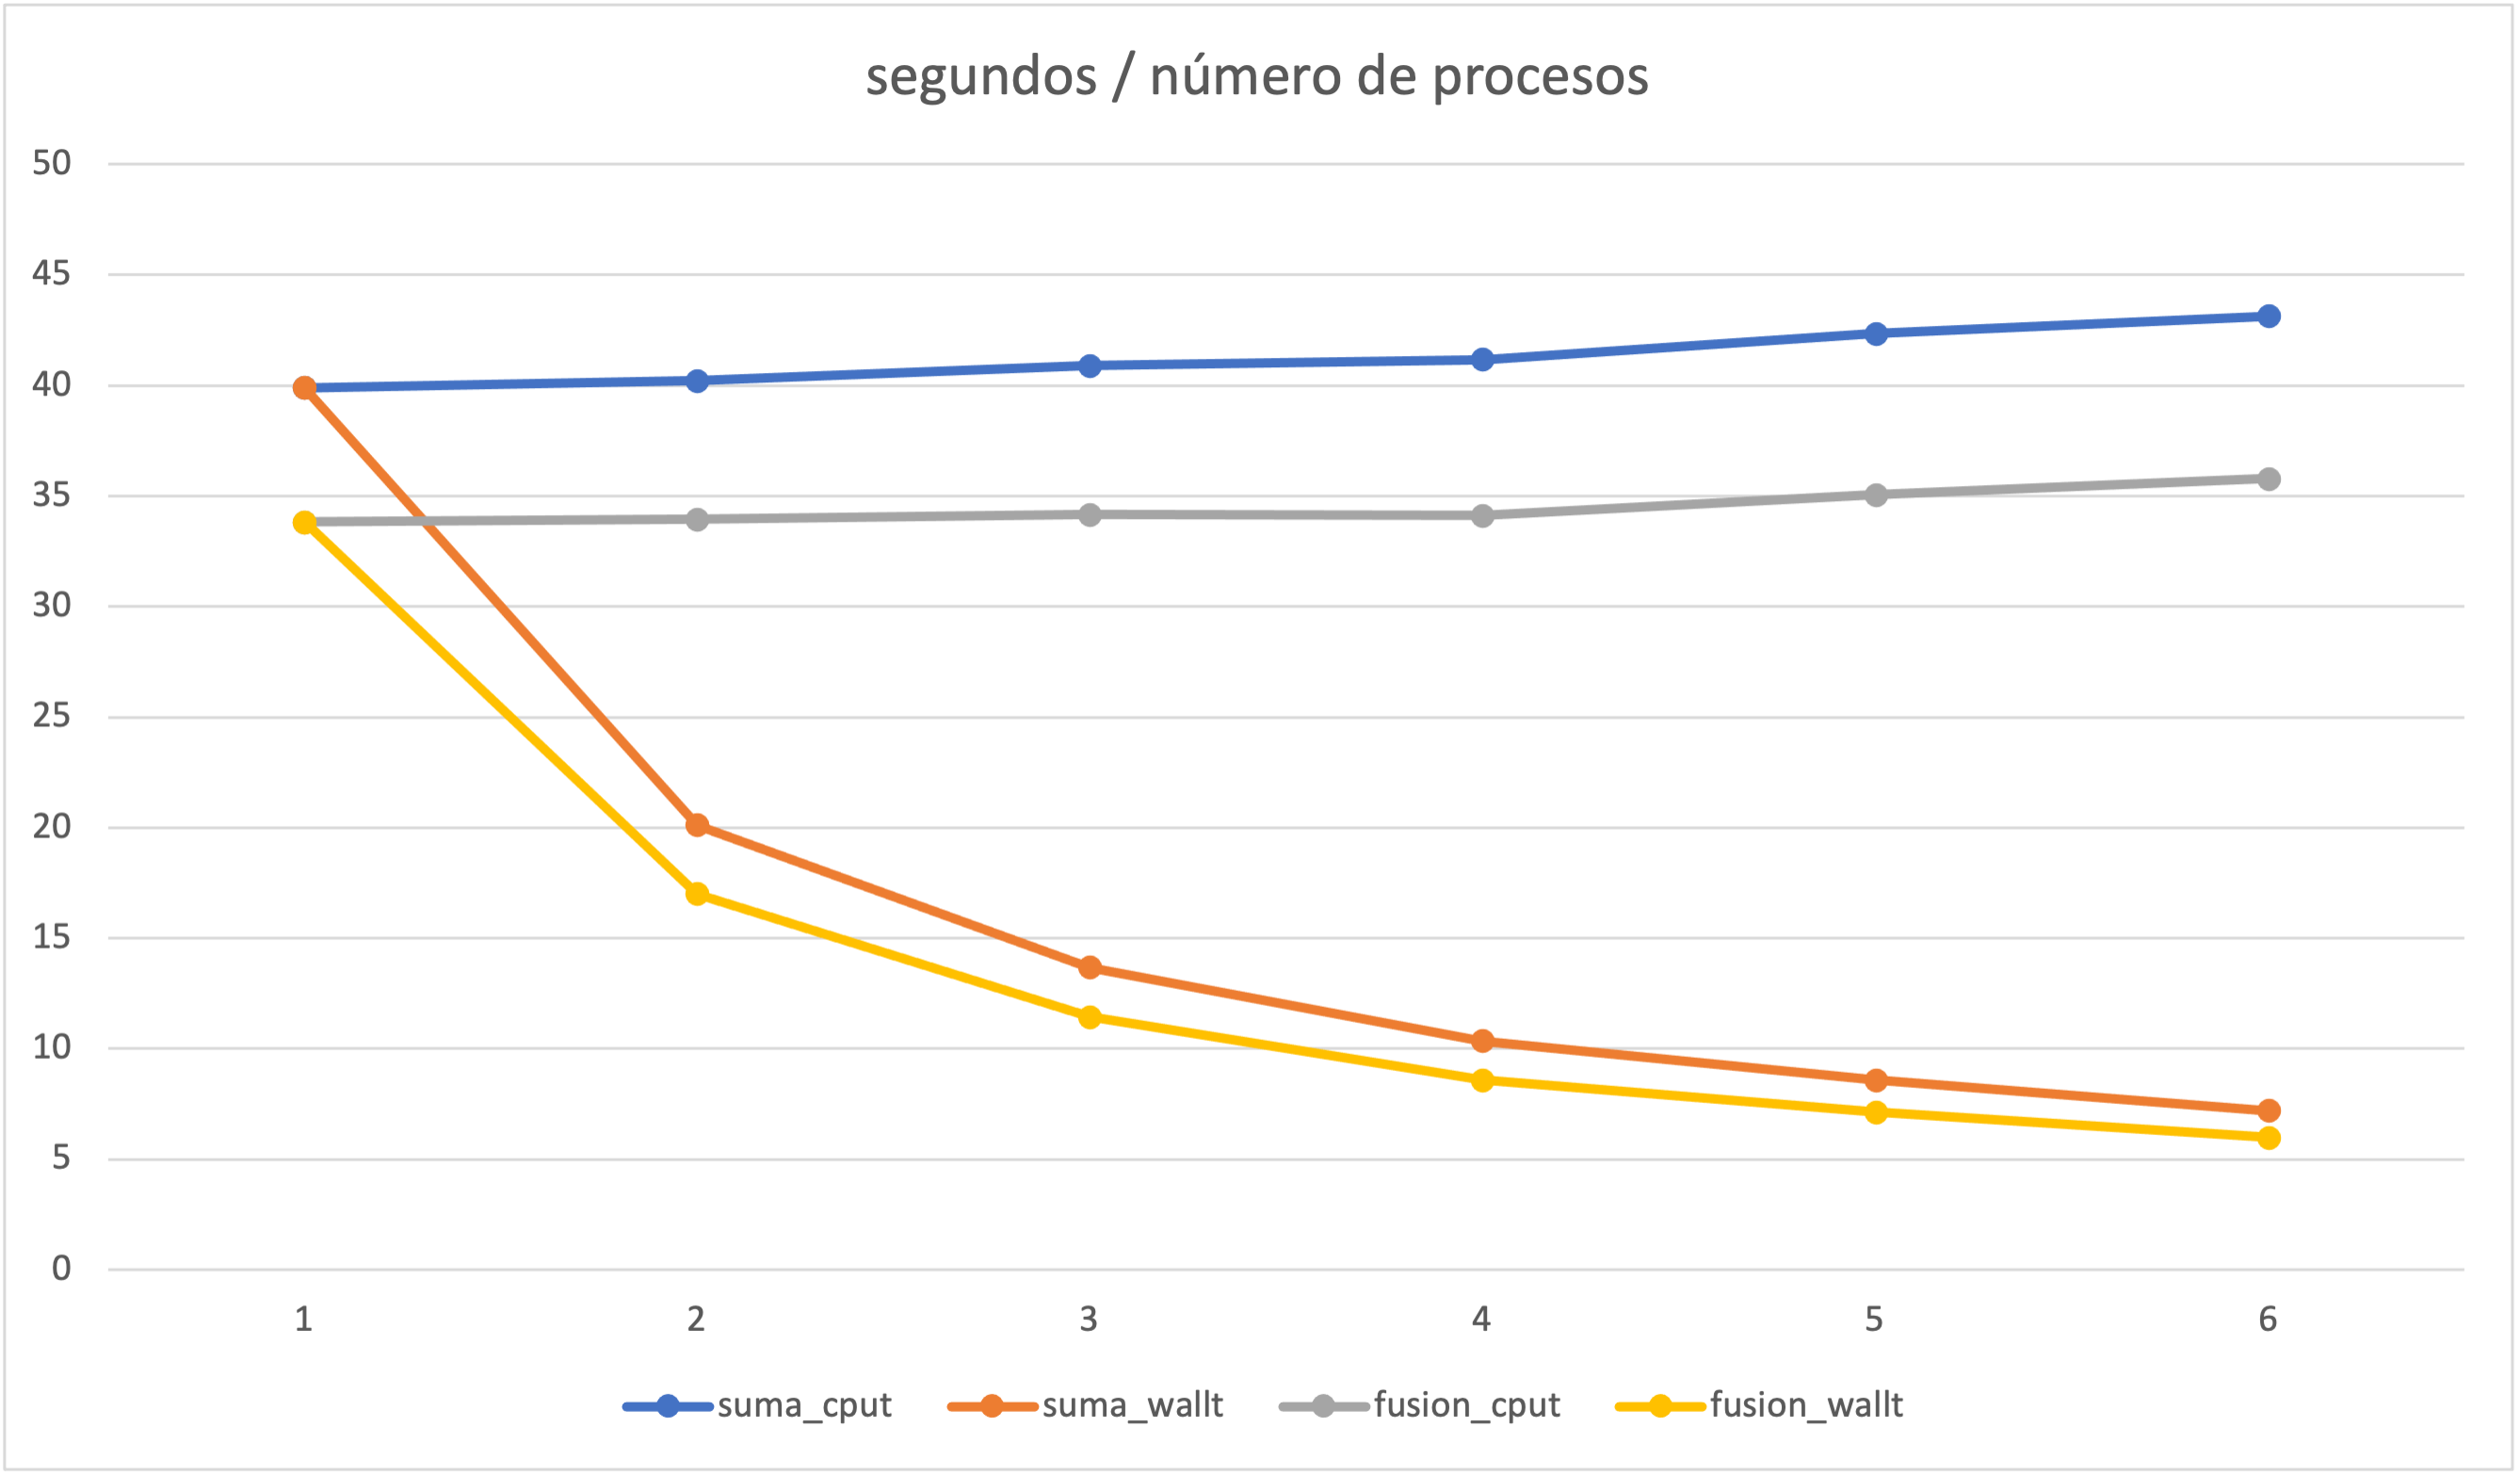
\includegraphics[width=16cm]{ap.png}
    \caption{Relación segundos / número de procesos. Observamos cómo los tiempos de ejecución para
    el algoritmo en que fusionamos ambos algoritmos son menores que la suma de los dos algoritmos ejecutándose
    por separado. Esto se debe a que se divide entre dos el tiempo que el procesador gasta controlando el bucle
    \texttt{for}.}
\end{figure}